\documentclass[11pt]{article}
%\usepackage{algorithm}
\usepackage[section]{algorithm}
\usepackage{algpseudocode}
\usepackage[version=3]{mhchem} % Package for chemical equation typesetting
\usepackage{siunitx} % Provides the \SI{}{} and \si{} command for typesetting SI units
\usepackage{graphicx} % Required for the inclusion of images
% \usepackage{natbib} % Required to change bibliography style to APA
\usepackage{amsmath} % Required for some math elements
\usepackage{wrapfig}
\usepackage{amssymb}
\usepackage{amsmath}
\usepackage{epstopdf}
\usepackage{sectsty}  % set font size for section
\usepackage[left=1.2cm, right=1.2cm, top=1.5cm, bottom=1.5cm]{geometry}
\usepackage{mathtools}
\usepackage{setspace}
\usepackage{enumerate}
\usepackage{titlesec}
% \usepackage[backend=bibtex,style=verbose-trad2]{biblatex}
\usepackage{biblatex}
% \bibliography{refs} 
\addbibresource{refs.bib} 
%************************** FIGURES*******************************
\newcommand {\bfig}[2] {\begin{figure}
  \centering
  \includegraphics[width=#2]{#1}}
\newcommand {\brotatefig}[2] {\begin{figure}[htbp]
                        \centerline {
                         \epsfig{figure={#1},clip=,angle=-90,width={#2}}}}
\newcommand {\bfigfirst}[2] {\begin{figure}[h]
                        \centerline {
                        \setlength{\epsfxsize}{#2}
                        \epsffile{#1}}}
\newcommand {\efig}[2]{ \caption{#2}
                        \label{fig:#1}
                        \end{figure}
                        \mymarginpar{fig:#1}}
\newcommand {\erotatefig}[2]{ \caption{#2}
                        \label{fig:#1}
                        \end{figure}
                        \mymarginpar{fig:#1}}
\newcommand {\rfig}[1]{Figure \ref{fig:#1}}


\titleformat*{\section}{\LARGE\bfseries}
\DeclarePairedDelimiter\ceil{\lceil}{\rceil}
\DeclarePairedDelimiter\floor{\lfloor}{\rfloor}
\sectionfont{\fontsize{11}{15}\selectfont}
\newcommand*\diff{\mathop{}\!\mathrm{d}}
\setlength\parindent{24pt}
\linespread{1.4}
\setlength\parindent{0pt} % Removes all indentation from paragraphs
\renewcommand{\labelenumi}{\alph{enumi}.}
\title{Introduction to Blockchian Technology: The Lottery DApp} % Title
\author{Kevin~Tung~(kt2126),~Cheng-Yu~Chen~(cc4805),~Yingjin~Sun~(yj3400)} % Author name
\date{\today} % Date for the report


\begin{document}
\maketitle
\section*{Abstract}
With the extreme rise in popularity of blockchain technology in recent years, there has also been a significant increase of decentralized applications (DApp) out in the market. Some of this include decentralized finance (DeFi), decentralized games, and even NFT trading platform. In our project, we would like to focus on the field of DeFi with our own addition of introducing a lottery capability to our DeFi platform. We will be first creating our own ERC-20 token called Lottery (LOT) in which will have a total supply of 750,000 tokens. Then, we will be creating a DApp that will allow users on the network to purchase the LOT token and utilize the lottery function. The lottery function will allow the user to pay a certain amount of CCN token to be entered into a pool with other users, in which a random generator will be used to choose the winner of the lottery. By adding the lottery function, we hope to add randomness to the allocation of LOT that will be fun for users to experience.
\section*{Introduction}
Our project is mainly split into three parts alongside a frontend and a backend component. The first part of our project is the creation of our ERC-20 token LOT and it is located in the LotToken.sol file. This file defines the smart contract that is needed to define the basic functions of LOT. Our smart contract follows the ERC-20 token standard as specified here \parencite{WEBSITE:1}. This standard provides basic functionality to transfer tokens as well as approving certain amount of tokens to be spent by another on-chain third party. By following the ERC-20 standard will also allow LOT to be re-used by other applications on the Ethereum network. In LotToken.sol, we first defined the constructor and defined the name, symbol, total supply, as well as a dictionary mapping of balanceOf and allowance to gather information of a certain wallet address. Then, we defined the transfer function which is responsible for transferring a specified amount of tokens to a specified address. Next, we defined the approve function which allows a spender to withdraw from another multiple time up to a specified amount of value. Lastly, we defined the transferFrom function which allows for the transfer of a specified amount of tokens form a specified address to a specified address. With all of these functions written, it sets up the backend foundation of the LOT token. \\
The second component of our project is responsible for the token sale of the LOT token including the backend and the frontend. The backend of the token sale can be found inside the LotTokenSale.sol file. Within this file, we first created the constructor which specifies the tokenPrice, tokenContract as well as tokensSold. Then, the main function in the LotTokenSale.sol file is the buyTokens function. This function allows any user on the Huygens network to exchange their CNN tokens for a specified amount of LOT token. Then, it also updates the total number of tokens left for sale to update it on our DApp for the token sale. Another important function inside this file is the endSale function, which allows the admin to end the sale of the token and transfer the unsold LOT tokens back to the admin. To allow the users to easily access the LOT token sale without any programming experience, we created a frontend on lite-server locally. The frontend is directly connected to our smart contracts in the backend. This simple frontend interface allows the user to easily purchase the LOT token, as well as see information such as the amount of LOT you currently have, amount of LOT tokens sold and your wallet address. An example of the frontend can be seen below in \rfig{fig1}.\\

\begin{figure*}[!t]
\centering
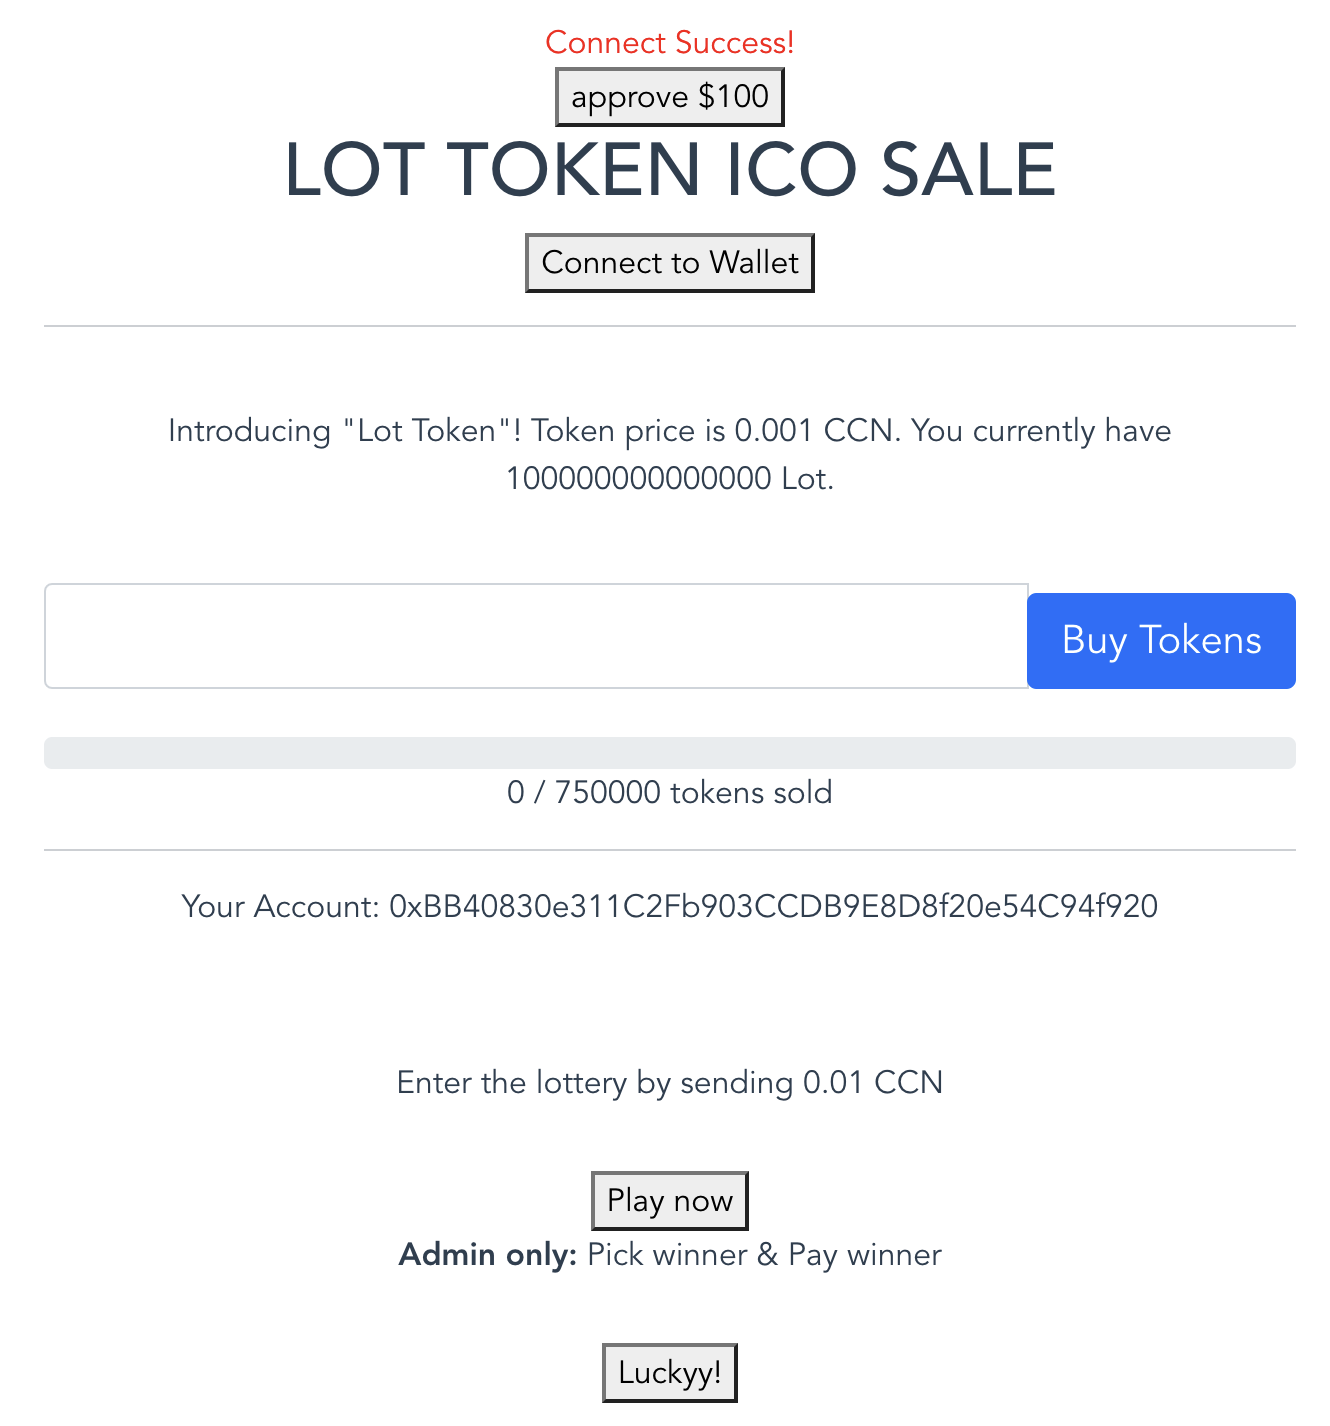
\includegraphics[width=3.5in]{figure1.jpeg}
\caption{Frontend of our DApp: Lot Token Sale.}
\label{fig:fig1}
\end{figure*}

The last component of our project is responsible for the lottery functionality of our DApp platform. The backend of the lottery functionality is located inside the Lottery.sol file. In this file, we created functions such as pickWinner, payWinner, enter, getWinnerByLottery and getPlayers. The workflow of the lottery function work as follows. First, the user will have to enter the lottery pool by paying a certain amount of CNN. Then, once there are enough players in the pool, the admin then uses the pickWinner function to pick the 1 winner inside the pool. Next, the payWinner function transfers all the token that was inside the lottery pool to the winner’s wallet address. As you can see below in figure 2 shows the frontend of the lottery function of our DApp which allows the user to easily interact with the lottery function within our DApp and to quickly understand the state of the current lottery pool.\\
\section*{Originality}
The main creative component of our DApp with the LOT token is the lottery functionality. Typically, we have seen DeFi tokens that have burning and staking capabilities to alter the supply of the tokens. However, we have yet to see a DeFi token that have a lottery capability as described above. By adding the lottery capability will introduce randomness to the token circulation that will incentivize users to participate in the LOT token ecosystem. We have seen how much of an impact randomness and luck can be made in real life examples such as a casino, therefore, we wanted to introduce a lucky component into our DeFi ecosystem with the LOT token. \\
Another component of originality is that we designed a user-friendly frontend for users to easily interact with the smart contract. By doing this, it allows users with no prior experience with DeFi platforms to easily trade the LOT token and to understand what actions they are currently doing. Furthermore, this also allows the users to easily use the lottery function to experience the unique component we have introduced. Having a user-friendly frontend definitely helps with getting more users on our DApp.\\
\section*{Showcase of our DApp}
In this section we will be showcasing the major components of the Lottery DApp. As seen below in figure 3 showcases the frontend of our DApp where the user can easily interact with the backend of our DApp with our user-friendly interface. On the top of the DApp there is a “Connect to Wallet” to connect your Ale wallet to our DApp and after the connection is successful it will also notify the user of this status. After the user has successfully connected to DApp, the user can now freely use any of the functions in our DApp. On top of the “Connect to Wallet” button, there is a “approve \$100” button which allows the user to test out our approval functionality. Next, there is a field which allows the user to purchase the LOT token for the price of $0.001$ CNN per LOT token. Furthermore, it also displays the total amount of LOT token sold up to this point along with how many LOT tokens the user owns. Below that, our DApp also displays the user’s Ale wallet address to confirm whether this is the correct wallet the user would like to interact with our DApp with. The bottom half of the DApp is the lottery functionality of our DApp. The first functionality is the “play now” button which allows the user to pay 0.01 CCN to participate in the current lottery pool. Below that, it displays the functionality that can only be operated by admins, which allows the admins to pick and pay the winner of the current lottery. Then, below that is the lottery history which clearly shows the winner of each previous lottery pool. Next, the DApp shows the current players in the lottery pool and the their wallet addresses. Lastly, the DApp displays the current pot size of the current lottery pool to let the users know how much they can possibly win from this lottery. Overall, our DApp is user-friendly and allows the user to clearly know the different functions and understand whether the action was successful or not. Furthermore, it also allows the users to know in real-time the current state of the LOT token ecosystem such as supply.
\section*{Conclusion}
Overall, our Lottery DApp showcased a platform that allows for user to buy the LOT token using CNN while enjoying the lottery functionality we have designed. We were able to create a user-friendly frontend website to integrate with the smart contracts on the backend. Our DApp is unique in that it introduces randomness with the lottery function to alter the supply and allocation of the LOT token. This deviates from the traditional token allocation of buying and selling or even burning. However, this also introduces a fun component for users to interact with the DApp that can result in them earning a lot of LOT token back with their luck. We believe that this lottery component will definitely intrigue users to try out our DApp and experience the LOT DeFi ecosystem.\\
I believe that we can continuing building upon the lottery concept with our DApp to further expand the Lottery DeFi ecosystem. Some of these functions can include live LOT token price tracking, token allocation chart and adding more features to introduce randomness into the LOT token supply. By doing so, it can definitely set up a more concrete foundation for the LOT ecosystem and attract more users to participate in our DApp. Another major component we can definitely improve on is the design of the frontend and the market the LOT token better. With a more user-friendly frontend along with advertising the DApp on different platforms, will definitely help with attracting more users to use our DApp. We hope to continue developing the future for the LOT token ecosystem and fully develop into a complete DeFi platform.

\newpage
\printbibliography[title=References]
\end{document}